\chapter{From Bloom filters to Bloomaps}

During points-to analysis the datastructure is almost as important as the
algorithm used. In the case of GCC, the structure chosen is a hybrid of bitmap
and a linked list. This works fine for small and dense data, but not so well
with large data. Converting to a better data structure is relatively easy task, but what data
structures are available? We will start by examining the needs of a typical
Andersen-style algorithm and comparing theoretical complexities of various well
known data structures. In the rest of this chapter we will describe a new
enhancement of bloom filters called Bloomaps, tailored specifically for the use
in points-to analysis.

\section{Requirements}

As a basic data structure for PTA, we need a data structure holding sets of
integers that is compact and has the following operations.

\begin{itemize}
	\item {\tt INSERT(set, element)} -- inserts {\tt element} into {\tt set} and returns if
		the structure has been changed by the insertion.
	\item {\tt QUERY(set, element)} -- checks if {\tt element} is part of {\tt set}.
	\item {\tt INTERSECTION\_EMTPY(set1, set2)} -- checks if intersection of {\tt
		set1} and {\tt set2} is empty.
	\item {\tt ENUMERATE(set)} -- lists all elements in a {\tt set}.
	\item {\tt UNION(set1, set2)} -- merge {\tt set2} into {\tt set1}.
\end{itemize}

The algorithm uses the following operations in the following way:

\begin{itemize}
	\item Initialization: {\tt INSERT} used to populate points-to sets with
		memory locations assigned to them.
	\item Propagation: {\tt UNION} for every copy constraint, {\tt ENUMERATE} and
		{\tt UNION} for dereferences.
	\item Oracle queries: {\tt QUERY} for set membership, {\tt INTERSECTION\_EMPTY}
		for set disjointness
\end{itemize}

In other words, the basic operations can be slower, {\tt
INTERSECTION\_EMPTY} and {\tt UNION} has to be fast. There are a few other considerations:

\begin{itemize}
	\item {\tt UNION} will be called on the same pairs over and over again,
		the difference will usually be in just a few elements.
	\item The average number of stored elements will be small, and the data sparse.
	\item Some sets may grow very large, containing almost every element possible.
	\item Low memory overhead is required, as the number of sets is in the order
		of number of elements inserted.
\end{itemize}

\TODO{Rozvest}
A simple bitmap is a straightforward solution, but the sparseness make it
unviable. Many tree-like structures will have problems with the intersections
and union as all the elements have to examined and deduplicated. Structures
requiring pointers, storing element values or hashes do have large overhead.

\section{Bloom filters}

A bloom filter is a classical probabilistic data structure, invented by Burton
Howard Bloom \cite{Bloom1970}. The goal is to provide a data structure
that has some nonzero probability of {\it false-positive}, but zero probability
of {\it false-negative}. This is accomplished by taking a bit field of $m$ bits,
$k$ hash functions, and hashing every element into $k$ different bits, writing
$1$ on insertion, and checking if every position contains $1$ on query.

The Bloom filter has immediate applications in some areas, for example caching:
it is a good idea to ask a filter if an element is in the cache. If the answer is
no, we need to get it elsewhere. If the answer is yes, we can look into the
cache, and in the worst case it is not there (an ocurrence false-positive).

Basic operations can be implemented with the following time complexity (provided
the hashes can be computed in constant time, which is often possible):

\begin{itemize}
	\item {\tt QUERY} in $\O(1)$ time.
	\item {\tt INSERT} in $\O(1)$ time.
	\item {\tt DELETE, ENUMERATE, RESIZE} not supported\footnote{Though there
		are variations that support these oprations, only {\tt RESIZE} is usually
		possible without drastic changes to the structure.}.
	\item {\tt UNION} in $\O(m)$ time (bitwise OR).
	\item {\tt BITWISE\_INTERSECTION} in $\O(m)$ time.
\end{itemize}

Unlike in simple bitmaps, bitwise intersection of bloom filters is not equal to
set intersection.  Denote by $BF(A)$ a bloom filter created from empty
filter by inserting elements from $A$ one by one. Then for $A,B$ it does not
hold that $BF(A \cap B) = BF(A) \cap BF(B)$. While the inequality $BF(A \cap B)
\subseteq BF(A) \cap BF(B)$ holds, it is nowhere near the equality. Most
imporantly {\tt INTERSECTION\_EMPTY} is hardly reasonably accurate, because a
single bit in {\tt BITWISE\_INTERSECTION} causes the filter to be non-empty. 

\section{Bloom filter intersection}

Although a bloom filter intersection easily computed with bitwise {\tt AND},
it is rarely accurate. As proven in \cite{bose2008false}, the probability that
$BF(A\cap B) = BF(A) \cap BF(B)$ is:

\begin{align*}
	p = (1-1/m)^{k^2\cdot |A-A\cap B| \cdot |B - A\cap B|} \mathrm{.}
\end{align*}

\noindent For {\tt INTERSECTION\_EMPTY}, we can further simplify the formula by
considering two cases: $|A \cap B| > 0$ and $|A \cap B| = 0$. Assuming that
$|A\cap B| = 0$, the probability that $BF(A) \cap BF(B)$ is also empty, is as
follows:
\begin{align*}
	p_{empty} = (1-1/m)^{k^2 \cdot |A| \cdot |B|}
\end{align*}

Jeffrey and Steffan \cite{Jeffrey2011} showed a slightly improved bound with
partitioned bloom filters.

\begin{align*}
	p_{empty} = \left(1 - \left( 1 - {k \over m}\right)^{|A|\cdot |B|}\right)^k \mathrm{.}
\end{align*}

Partitioned bloom filter has a separate partition for each hash function of size
$m/k$, therefore it is enough to have one empty partition to consider the filter
empty, as every query would result in false in this empty partition.

The same paper also proved that pure Bloom filter intersection is more
memory consuming than more conventional queue-of-queries. In the next section,
a hybrid solution is provided that can be used with both of these approaches,
based on the time requirements.

\section{Bloom filter enumeration}

It is immediately clear that vanilla Bloom filter does not support element
enumeration. For example the simplest filter holding $1$ elements and
answering with false-positive probability $0.5$ would have to enumerate half the
universe $U$, which may as well be impossible for $U=\N$.

Let us briefly summarize a few options most commonly used:

\paragraph{Enumerate entire universe.} Without any extra information on what
may be contained in a filter, we have to check for every element in the
universe. This is possible for small and dense universe, and appropriately sized filter.
Even for almost empty filter, this approach takes $\O(|U|)$ time.

\paragraph{Keep a Queue-of-queries for each filter.} This approach is suggested
by \cite{Jeffrey2011}. We keep a queue of elements inserted into the filter,
which is evaluated in case the elements need to be enumerated. The queue usually
holds each element as many times as it has been inserted. The filter has
limited capacity, so as long as we do not insert elements many times over
excessively, the list can not grow indefinitely. However, this approach does not
work well with {\tt UNION}, as the lists would have to be either concatenated
(in which case the lists would grow exponentially) or pruned after each union,
which would be essentially same as using bitmaps.

\paragraph{Alternative structures.} An alternative structure has been proposed,
the Invertible Bloom
Lookup Tables (IBLT), by Michael T. Goodrich \cite{goodrich:2011}. The problem of IBLT is
that they have non-zero probability of being unable to produce a complete list
of entries, and do not provide the advantages of classic Bloom filters, as a
fast intersection and membership queries. This said, we will not attempt to use
them, although they are an interesting structure for future work and may find
its use in other optimizers.

Neither of these methods are good for use in points-to analysis, as our universe
can be large (millions of lines of code), and the number of filters is about the
same size as the universe. We introduce a new approach, a compromise between the
two above.

\paragraph{Keep a single Queue-of-queries for all filters.} The number of sets
in PTA prohibits the use of queue-of-queries for each filter. The universe
enumeration could be used, but is wasteful as only some variables will ever be
inserted in the set. However, we can keep a global queue-of-queries for all
filters used in the algorithm. Each element inserted will be recorded in an
indexed data structure, and parts of this structure will be searched and
evaluated later, when enumeration is requested.

Choosing a good data structure is still important, as we still need low overhead
and preferably fast insertion. Assuming our universe is all 32 bit integers, a
single bit array of every item ever inserted in under 512 MB. This is
reasonable, but storing even 8 bits for each element would result in 4 GB, which
is not. We show later in this chapter an efficient indexed bit array with
insertion in $\O(1)$.


\section{Bloomaps and Families}

{\it Bloomap Family} with parameters $(m, k, s)$ is a datastructure that
maintains a list of Bloomaps of the same parameters, and indexed representation
of used parts of the universe in union of all its Bloomaps, capable of
enumeration.

A {\it Bloomap} is an enhanced Bloom filter, belonging to a single
family, capable of executing {\tt INSERT} and {\tt QUERY} itself, and {\tt
ENUMERATE}, {\tt UNION} and {\tt INTERSECTION} within its family.

Bloomap with parameters $(m, k, s)$ is constructed from a partitioned Bloom
filter with $k$ partitions, each for one hash function, with the addition of a
{\it side index} containing $s$ bits. The side index is used as another
partition in the Bloom filter, however with simpler hash function that is easily
inverted (for example a simple {\tt SHIFT} and {\tt AND} with a mask).

Furthermore, the Bloomaps and their families need to fulfill these conditions:

\begin{itemize}
	\item When a new item is inserted into a Bloomap, it is also inserted into
		the family.
	\item A Family has to enumerate all items inserted into it's Boomaps for any
		given hash.
\end{itemize}


Figure \ref{figure-bloomap-decl} shows Bloomap and BloomapFamily prototypes.
Here {\tt hash\_set} is some data structure capable of storing a set of
elements from universe associated with a given hash. In C++, {\tt
hash\_map<vector<universe\_type>>} could be used as a naive data structure, but
we offer a better solution later in this chapter. See Figure
\ref{figure-bloomap-fn} for pseudocode implementation of {\tt INSERT} and {\tt
ENUMERATE} functions. Overview of Bloomap structure is shown in Figure
\ref{figure-bloomap-overview}.

\begin{figure}[!ht]
\centering
	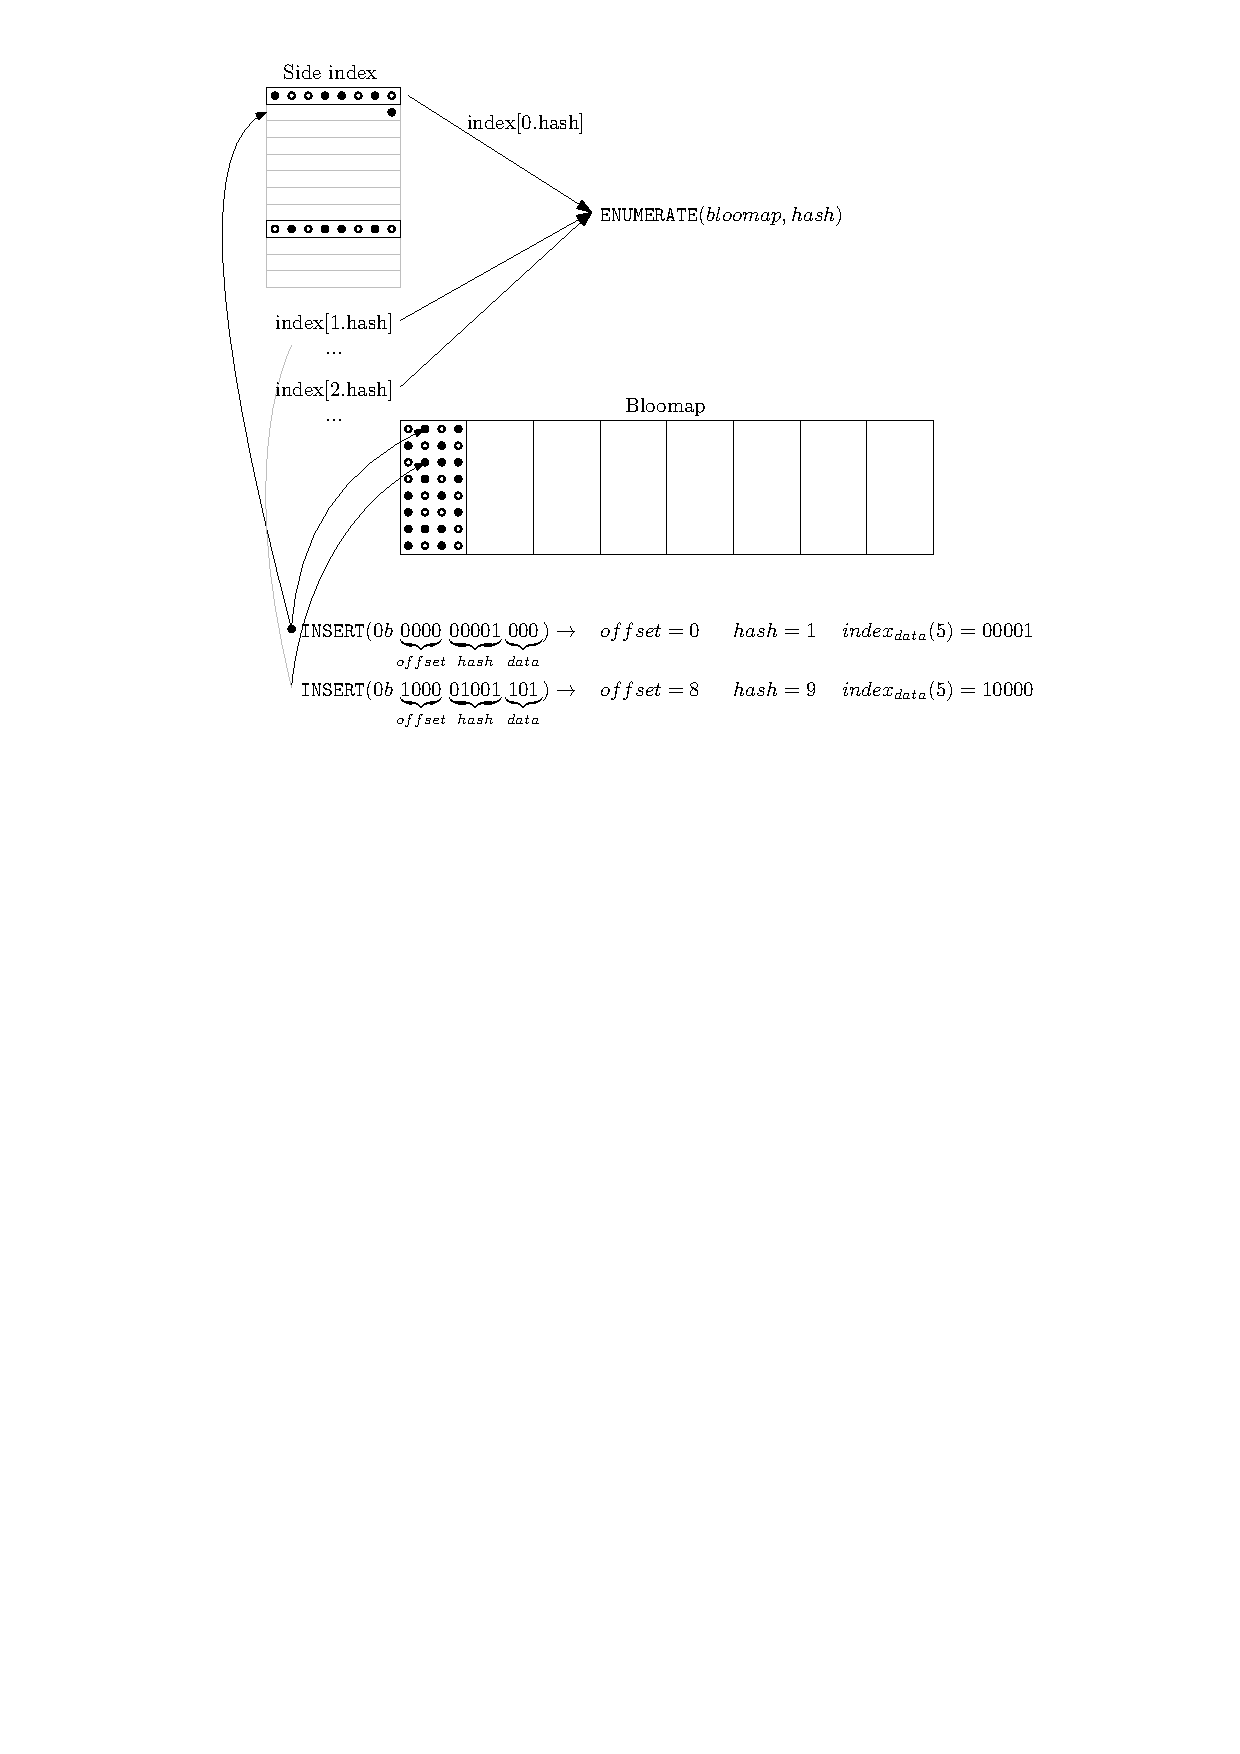
\includegraphics{./img/bloomap_overview.pdf}
	\caption{Overview of Bloomap structure}
	\label{figure-bloomap-overview}
\end{figure}



Both of them are pretty straightforward, as {\tt INSERT} is a regular function
for Bloom filter insertion, with the added partition for side index and family
universe insertion.

While insertion in Bloom filter is in $\O(1)$, inserting into a universe may be
$\O(\log n)$ for tree-based implementations or amortized $\O(1)$ for hash-based
implementations. There probably is not a better solution in generic case,
but we suggest a worst-case $\O(1)$ for 32 bit integers (dense sequence of
ids starting from 0).

The Bloomap achieves the following theoretical complexity:

\begin{itemize}
	\item {\tt QUERY} in $\O(1)$ time.
	\item {\tt INSERT} in $\O(1)$, assuming $\O(1)$ insertion into universe
		index.
	\item {\tt DELETE{\rm ,} RESIZE} not supported.
	\item {\tt ENUMERATE} in $\O(|U|)$ in worst case, assuming universe index
		suggested in section \ref{sec-compact-representation} and $|U|$ the size
		of the index.
	\item {\tt UNION} in $\O(m)$ time.
	\item {\tt BITWISE\_INTERSECTION} in $\O(m)$ time.
\end{itemize}

\subsection{Compact representation of dense integer universe}
\label{sec-compact-representation}

Representing universe requires storing sets for different hashes. It is wasteful
to store them in a linked-list, trees or even hash tables, as a humble bit array
fulfills the task. A little unusual form of a bit array has been used, in order
to achieve less allocations and good space efficiency.

As mentioned above, we will split the value to {\tt offset}, {\tt hash} and {\tt
data} at binary boundaries. This means we can simply concatenate the values to
get the represented integer. We can now organize the data into {\it buckets} and
{\it superbuckets} in the following way:

\begin{itemize}
	\item Each {\tt offset} has it's own {\it superbucket}.
	\item Each {\it superbucket} contains a {\it bucket} for every {\tt hash} value.
	\item Each {\it bucket} contains a bit for every {\tt data} value.
\end{itemize}

\begin{center}
	{\tt element = offset$\cdot$hash$\cdot$data} $\Leftrightarrow$
	{\tt universe[offset$\cdot$hash].bit[data]}
\end{center}

\begin{figure}[h!]
	\centering\hspace{2.5cm}
	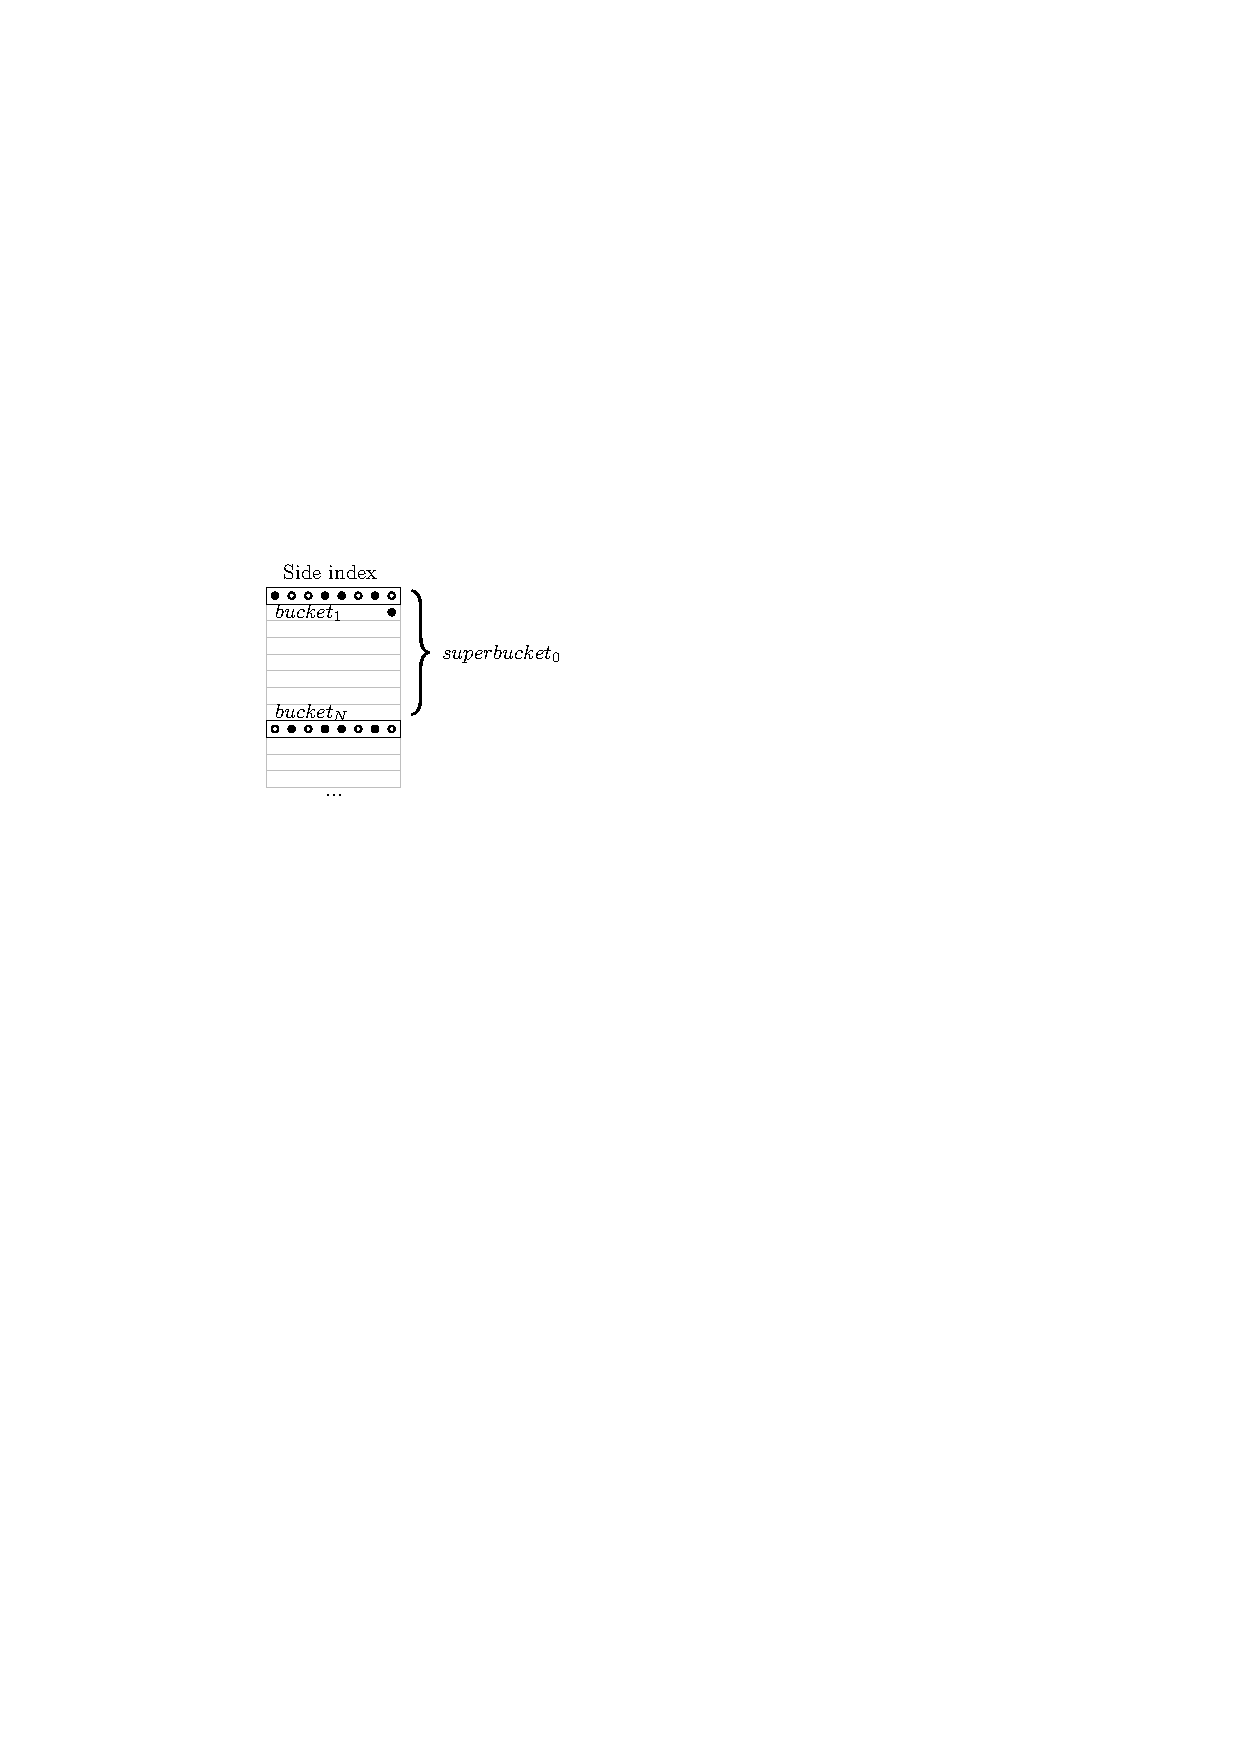
\includegraphics{img/bucketshop.pdf}
	\caption{Bucket and superbuckets in an array.}
	\label{figure-bucketshop}
\end{figure}

The structure is illustrated in Figure \ref{figure-bucketshop} and pseudocode
implementation in Figure \ref{figure-bucketshop-pseudocode}. Memory allocation
is expected to be done automatically in {\tt vector} class and the array should
be resized on first access beyond current boundary.  This allows the structure
to occupy only as much memory as is necessary to store a set of size at most
$\O(\max(E))$, where $E$ is the number of elements inserted. In this case, a
bucket has 64 bits, so it will fit up to 6bit data. Number of bits in hash and
offset is not important and should be chosen by the size of Bloomap's side
index.

\begin{figure}[h!]
\begin{tcolorbox}
\begin{verbatim}
struct superbucket {
  uint64_t bits[];
};

struct universe_index {
  vector<struct superbucket> superbuckets;
};

void universe_index::INSERT(offset, hash, data) {
  superbuckets[offset]->bits[hash].bit[data] = 1;
}

vector<element> universe_index::ENUMERATE(hash) {
  vector<element> candidates;
  for (sb in superbuckets) {
    for (i = 0 .. 63) {
      if (sb->bits[hash].bit[i]) 
        candidates.append(bit);
    }
  }
  return candidates;
}
\end{verbatim}
\end{tcolorbox}
\caption{Bucket and superbuckets prototype and pseudocode}
	\label{figure-bucketshop-pseudocode}
\end{figure}

\begin{figure}[!ht]
\begin{tcolorbox}
\begin{verbatim}
struct Bloomap {
  BloomapFamily f;            # Family this maps belongs to
  int m,k,s;                  # Filter parameters

  int index[s];               # Side index
  int partitions[k][m/k];     # Regular filter partitions
};

struct BloomapFamily {
  vector Bloomap;             # Owned bloomaps
  int m,k,s;                  # Filter parameters

  hash_set universe;          # Indexed universe
}
\end{verbatim}
\end{tcolorbox}
\caption{Bloomap and BloomapFamily prototypes}
\label{figure-bloomap-decl}
\end{figure}

\begin{figure}[!ht]
\begin{tcolorbox}
\begin{verbatim}
bool Bloomap::QUERY(element) {
  for (i := 1..k) {
    if (partitions[i][hash_fn(i,element) % m/k] == 0)
      return false;
  }
  return true;
}

void Bloomap::INSERT(element) {
  # Decompose element to offset, index_hash and data.
  (offset,index_hash,data) := element;
  # Insert into side index of a bloomap.
  index[index_hash] := true;
  for (i := 1..k) {
    partitions[i][hash_fn(i,element) % m/k] := 1
  }
  # Insert into universe index of a family
  f.universe[index_hash] += element;
}

void Bloomap::UNION(another) {
  for (i := 1..s) {
    index[i] |= another.index[i];
  }
  for (i := 1..k, j := 0..m/k) {
    partitions[i][j] |= another.partitions[i][j];
  }
}

vector Bloomap::ENUMERATE() {
  vector list = ();
  for (i := 1..s | index[i] == true) {
  	for (element in f.universe[i] && this.QUERY(element)) 
      list += element;
  }
  return list;
}

\end{verbatim}
\end{tcolorbox}
\caption{Pseudocode for basic Bloomap operations}
\label{figure-bloomap-fn}
\end{figure}
